\chapter{Namespace XML}

Les documents XML bien formés répondront à l'arborescence présentée ci-dessous.

Les hypothèse suivantes sont également formulées :
\begin{itemize}
    \item Les documents XML à parser ne contiendront pas de DTD interne
    \item Les Process Instruction (PI) ne contiendront que des attributs
    \item Aucune référence ne sera présente dans les documents XML\\
\end{itemize}


\section{Diagramme de classes}
    Les classes ici décrites seront rattachées au \lstinline$namespace Xml$ défini en C++.

    \begin{landscape}
    \begin{figure}[h!]
        \centering
        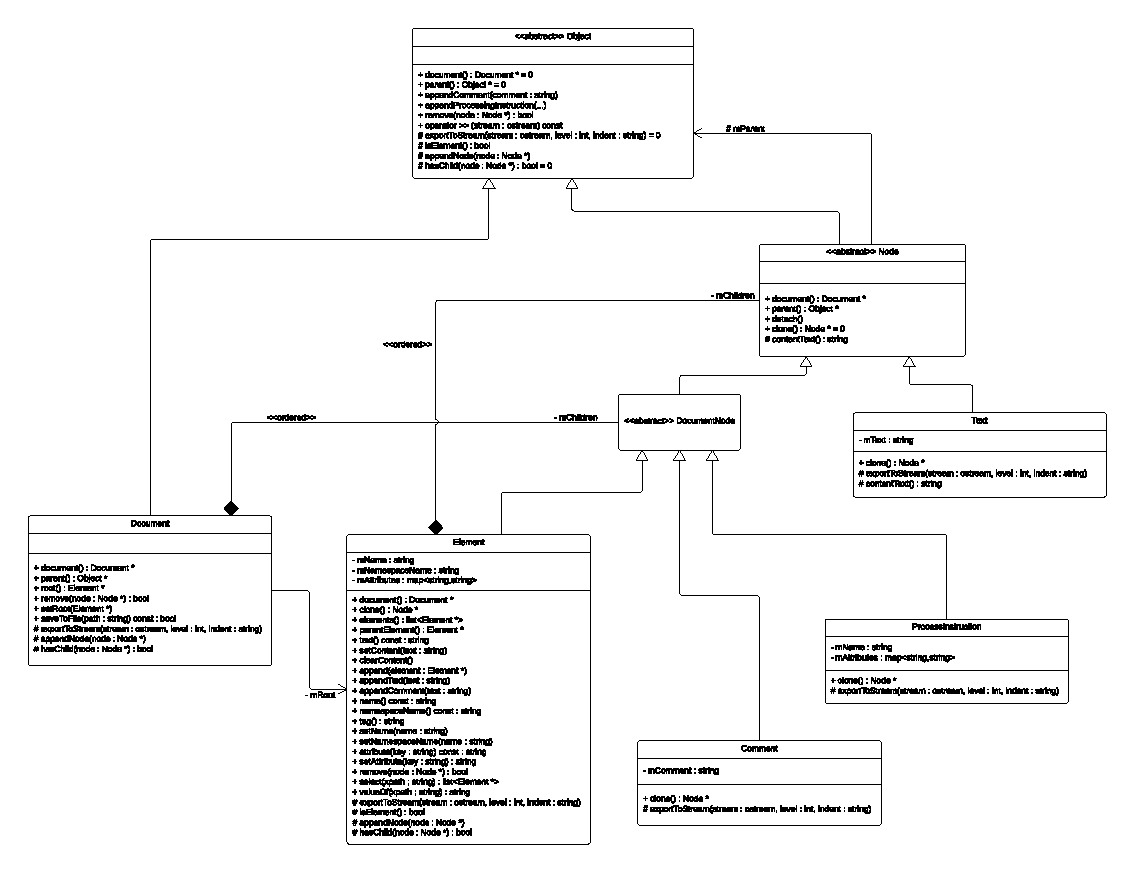
\includegraphics[width=0.9\linewidth]{images/xml-uml.pdf}
        \caption{Diagramme de classes de l'arborescence XML}
        \label{classDiagram}
    \end{figure}
    \end{landscape}


\section{Classes}
    \subsection{Log}
        La class \lstinline$Log$ a pour unique mission de stocker l'ensemble de l'output du parseur \textit{XML} telle que~:

        \begin{itemize}
            \item Erreurs lexicales~;
            \item Erreurs syntaxique~;
            \item Erreurs semantiques.
        \end{itemize}

    \subsection{Object}
        Pour optimiser et eviter au maximum la redondance de donner dans notre arbre d'h\'eritage de l'implementation \textit{XML}, nous nous somme inspirer de la tres c\'elebre librarie \textit{Qt} avec sont \lstinline$QObject$. Ainsi nous avons notre \lstinline$Xml::Object$ offrant les avantages que vous trouverez dans les sous sections suivantes.

    \subsection{Node}
        Ainsi, nous partons du principe qu'un document XML n'est en faite qu'un arbre aillant des noeux (\lstinline$Node$) \'etant des objects XML, mais de natures differents (commentaires, text, element ...). Certains de ces noeux serons des feuilles de l'arbre pour le noeux de commentaire par exemple.

        C'est la d\'ej\`a un avantage du \lstinline$Xml::Object$ car chaque \lstinline$Node$ connais sont \lstinline$Object$ parent \'a l'aide de \lstinline$mParent$ pouvant etre un \lstinline$Element$ ou un \lstinline$Document$. Ainsi, on peut \'a partir d'un noeud, retrouver le \lstinline$Document$ dans lequel il se trouve simplement en remontant l'arbre.

    \subsection{DocumentNode}
        Le \lstinline$DocumentNode$ est une sp\'ecialisation de \lstinline$Node$, mais aillant seulement une particularit\'e' s\'emantique~: seul ses classes fillent peuvent avoir pour parent, un \lstinline$Element$ par hertiage de \lstinline$Node$, mais aussi un \lstinline$Document$ au contraire de la classe \lstinline$Text$ ne pouvant avoir pour parent qu'un \lstinline$Element$.

    \subsection{Document}
        Un \lstinline$Document$ est un \lstinline$Node$ aillant une composition de \lstinline$DocumentNode$. Parmis ces \lstinline$DocumentNode$, un seul et unique \lstinline$Element$ racine compose cette liste. Mais afin de pouvoir retrouver cette racine du document en complexit\'ee $O(1)$, \lstinline$DocumentNode$ dispose aussi d'un attributs \lstinline$mRoot$ dedi\'e \`a cette tache.

        Cette m\^eme liste de \lstinline$DocumentNode$ est ordonn\'ee pour pouvoir garentir l'ordre des noeux au chargement et \`a l'export du document \textit{XML}. L'\lstinline$Element$ racine compose cette liste pour eviter de gerer deux listes de noeux (ceux avant et ceux apr\`es).

    \subsection{Comment}
        \lstinline$Comment$ est un \lstinline$DocumentNode$ car il peut \^etre n'importe ou dans le document \textit{XML}~: dans un \lstinline$Element$ ou bien en dehors de l'element racine du document.

    \subsection{ProcessingInstruction}
        Une \lstinline$ProcessingInstruction$ est aussi un \lstinline$DocumentNode$ d'apr\'es les specifications officiel de \textit{XML}. Mais en accord avec l'hypothèse énoncée précédemment, une \lstinline$ProcessingInstruction$ ne contient qu'un nom et une map d'attributs.

    \subsection{Text}
        Un noeud de texte est naturellement décrit par une chaîne de caractères \lstinline$mText$. Celui-ci ne dérive pas de la classe \lstinline$DocumentNode$ puisque, si son contenu s'apparente à celui d'un noeud Comment, il ne peut en revanche être contenu par une instance de \lstinline$Element$. D'ou la nécessit\'ee d'ajouter le niveau de spécialisation \lstinline$DocumentNode$ afin d'éviter une relation ne respectant pas les sp\'ecifications standart \textit{XML}.

    \subsection{Element}
        Un \lstinline$Element$ \textit{XML} est un \lstinline$DocumentNode$ car il poss\`ede une liste d'\lstinline$Element$ enfant \lstinline$mChildren$, mais aussi peut l'\lstinline$Element$ racine d'un \lstinline$Document$.

        Celui ci est defini avec un nom de balise (\lstinline$mName$) mais aussi d'un espace de nom (\lstinline$mNamespaceName$). La concatenation de ces deux derniers forme le tag de l'\lstinline$Element$. Le nom du membre \lstinline$mNamespaceName$ au lieu de \lstinline$mNamespace$ a \'et\'e effectuer pour eviter la colision avec le mot clef du language C++ \lstinline$namespace$ avec son getter th\'eorique \lstinline$Xml::Element::namespace()$ remplacer par \lstinline$Xml::Element::namespaceName()$.

        Un \lstinline$Element$ possede un ensemble non-ordonné d'attributs etant simplement une map aillant une assossiation $clef \leftarrow valeur$, par soucis de determinisme, nous les exportons par ordre alphabetique des clefs.
